%!TEX program = xelatex
\documentclass[9pt, compress]{beamer}
\usetheme[titleprogressbar]{m}

\usepackage{booktabs}  
\usepackage[scale=2]{ccicons}
\usepackage{minted}
\usepgfplotslibrary{dateplot}
\usemintedstyle{trac}
\title{Community-PageRank: An efficient pipeline to predict communities to users}
\subtitle{{\normalsize Based on \emph{Beyond Friendship and Followers: The Wikipedia Social Network}\\by\\\emph{Johanna Geiss et al}}}
\author{Vaibhav Sinha, Vishwak S., Chandra Kiran Evuru\\
\texttt{CS15BTECH110\{34, 43, 12\}}}
%\subject{}
%\setbeamercovered{transparent}
%\setbeamertemplate{navigation symbols}{}
\begin{document}
	\maketitle
	

\begin{frame}[fragile]
  \frametitle{Review of earlier work}
\begin{itemize}
  \item \textbf{Goal:} Extract a large-scale person-centric 	network structure form English Wikipedia.
  \item Persons mentioned on a Wikipedia page have a common context, closer the names more evident the relationship.
  \item Wikidata contains data about 1.2M persons.
  \item Extracting persons based on Inter-Wiki Link (IWL) and drawing edges based on co-occurrences and distance, obtain a person network of roughly 800k persons and 67M edges.
  \item Identify centrality, clustering coefficients and component sizes.
  \item Also identify interesting communities and evaluate them .
  
\end{itemize}
\normalsize
\end{frame}

\begin{frame}[fragile]
	\frametitle{Recognition of persons in Wikipedia}
\begin{itemize}
\item Wikipedia (WP) contains 5.29M content pages, about 65M sentences. \footnote{As on January 12, 2015}
\item Classify a WP page as a person page based on year of birth and death, results in 1.05M pages.
\item To find references to persons in all Wikipedia page, a two step process is used, first following IWLs and then searching for 	recognized person names.
\item English WP has 76.8M IWLs of which 13.6\% (~10.4M) refer to persons. 99.9\% of these are identified by WD.
\item Search each page for persons that are already referred to in an IWL on that page.
\item About a third of pages that link to a person page also contain references to persons outside IWLs.
\end{itemize}
\end{frame}

\begin{frame}[fragile]
	\frametitle{Following interwiki links (IWLs)}
IWL is of the form [[\textit{linkTarget}|\textit{coveredText}]], where \textit{coveredText} is optional.
\begin{figure}
  \centering
 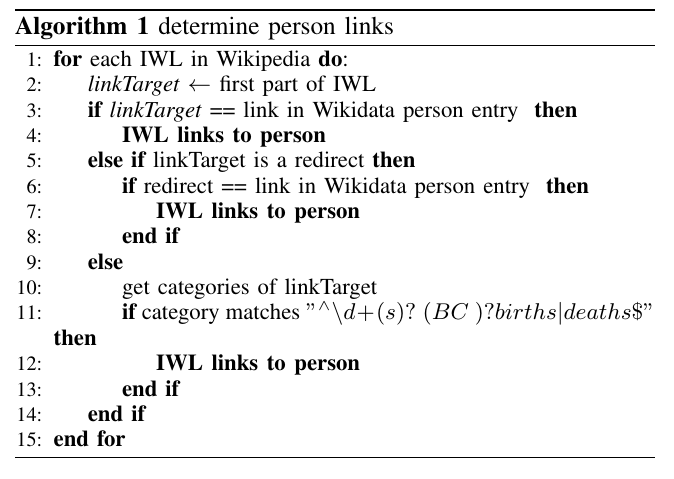
\includegraphics[width=7cm,height=5cm]{img/Algo1.png}
\end{figure}
\end{frame}

\begin{frame}[fragile]
	\frametitle{Person-Centric Network Construction}
\begin{itemize}
\item The network is represented in the form of a bipartite graph \(G = (V \cup D,E)\), where
\begin{itemize}
\item \(V\) : Set of nodes corresponding to people.
\item \(D\) : Set of nodes corresponding to the Wikipedia documents.
\item \(E\) : Set of edges \((u,p)\) such that \(u \in V\) and \(p \in D\) and iff document \(p\) contains person \(v\).
\end{itemize}
\item To construct a network of persons, we project graph \(G\) onto the set of persons.
\item We create a multi-graph as projection for each co-occurence between two persons as a single edge and then aggregate the edges to obtain a graph w/o multiple edges.
\end{itemize}
\end{frame}

\begin{frame}[fragile]
	\frametitle{Person-Centric Network Construction}
\begin{itemize}
\item Weights of edges in the multi-graph are given by : 
\begin{equation} \varphi(e = (v, w, i)) := e^{-d(v,w,i)/2} \end{equation}
\begin{itemize}
\item \(v,w\) : Belong to the set of persons.
\item \(i\) : Instance of a co-occurence between v and w 
\item \(d\) : Distance between v and w measured as the number of sentences between v and w in the documment that corresponds to i'th co-occurence.
\end{itemize}
\item To convert into a graph with single edges b/w two persons we aggregate multiple edges by cosine similarity of neighbourhoods for the two nodes.
\end{itemize}
\begin{equation}
dicos(v,w) = \frac{\sum_{e\in n_v \cap n_w} \varphi(e)^2}{\sqrt{\sum_{e\in n_v} \varphi(e)^2}\sqrt{\sum_{e\in n_w} \varphi(e)^2}}
\end{equation}
\end{frame}

\begin{frame}[fragile]
	\frametitle{Network Properties}
\begin{itemize}
\item The aggregated network contains exactly \(67, 583, 553\) edges, which connect the \(799, 181\) persons of which \(\approx 98.8\%\) is contained in one giant component / cluster.
\item Such a large network will cause inefficient future-processing such as community detection or finding network centrality.
\item Based on 5 structural metrics, choose a threshold of 0.0019 for edge weights to retain the edges in the graph.
\item \texttt{dicos} weighting helps by minimizing outliers and shortening the long tail.
\item The authors finally end up with a graph having $\sim$ 65 M edges and $\sim$ 800K nodes.
\end{itemize}
\end{frame}

\begin{frame}[fragile]
	\frametitle{Finding network centrality}
\vspace{-5mm}
\begin{itemize}
\item The PageRank centrality is used to find out the centrality of the network, which in this case is a group of people in the network.
\begin{figure}
	\centering
    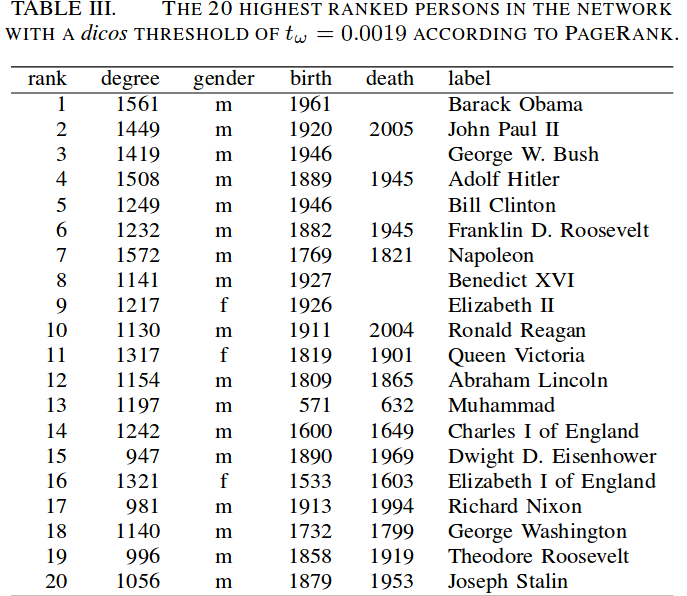
\includegraphics[width=0.7\linewidth]{img/network-centre.png}
\end{figure}
\end{itemize}
\end{frame}

\begin{frame}[fragile]
	\frametitle{Community Detection}
\vspace{-5mm}
\begin{itemize}
\item To detect the communities, the SLPA (stabilized label propagation algorithm) is used.
\end{itemize}
\begin{figure}
	\centering
    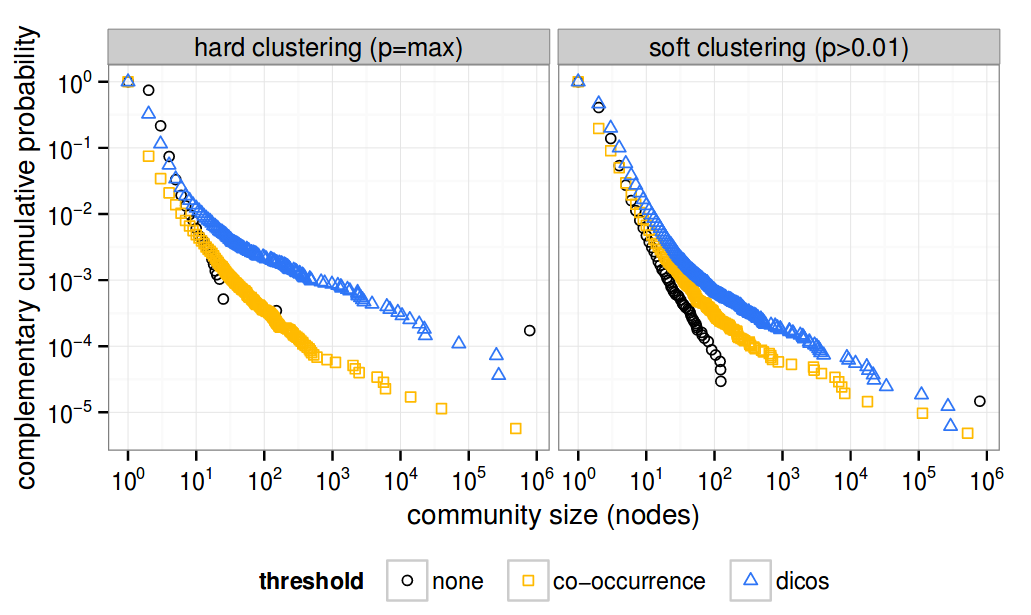
\includegraphics[width=0.8\linewidth]{img/comm-pdf.png}
\end{figure}
\begin{center}
Here the number of propagations made through the network is equal to 100. Note that the number of medium sized communities discovered is higher for the network obtained using \texttt{dicos} thresholding.
\end{center}
\end{frame}

\begin{frame}[fragile]
	\frametitle{Evaluation results and some discussion}
\vspace{-10mm}
\begin{figure}
	\centering
    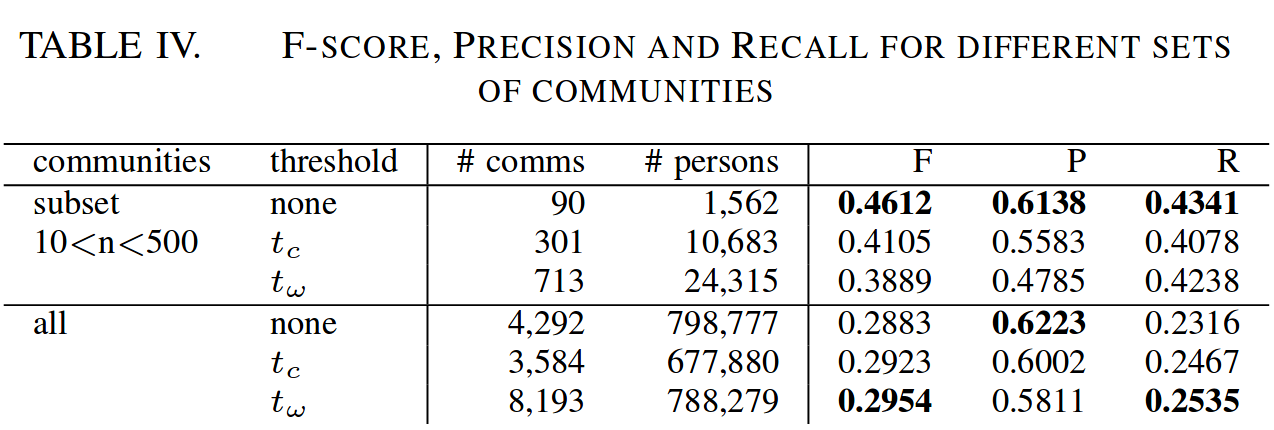
\includegraphics[width=0.75\linewidth]{img/table-eval.png}
\end{figure}
\begin{itemize}
\item This is entirely dependent on the policies of categorization which keeps changing.
\item This is also dependent on the scheme of thresholding used.
\item Hierarchical organization of categories in Wikipedia is a factor to be taken into consideration : to upto what level of hierarchy should we consider?
\item Semantically equivalent groups were identified, yet Wikipedia did not have that as a category.
\end{itemize}
\end{frame}

\begin{frame}[fragile]
	\frametitle{Our contributions}
\vspace{-10mm}
\begin{itemize}
\item Verification of statistics presented in the graph - both full and thresholded.
\item Verification of the results presented in the paper on the WSN (Wikipedia Social Network) - where we identify the top people from the network, detect communities in the network.
\item Community-PageRank Pipeline : Identifying top people in communities, and recommending new pages a community they ``might" belong to from the communities that were detected.
\begin{itemize}
\item We test this on three versions of the original graphs - discussion later...
\end{itemize}
\end{itemize}
\end{frame}

\begin{frame}
	\frametitle{Verification of statistics of the graph}
\begin{itemize}
\item The paper presents several statistics on the graph like the distribution of genders, occupation, year of birth e.t.c.
\item Obtained gender distribution (84.09\%, 15.81\%) is close to (84.3\%, 15.6\%).
\item Percentage of data having data birth: obtained 82.23\%, while reported value 83\%.
\item Similarly even for distribution of occupation we are able to get similar results.
\item Minor deviations from the reported value is probably from the difference in the graph used by the paper and the dataset which we worked with.
\end{itemize}
\end{frame}
% Insert the 2nd point thingy

\begin{frame}
	\frametitle{Visualizing the dataset}
\begin{figure}
	\caption{Variation of the size of categories}
	\centering
    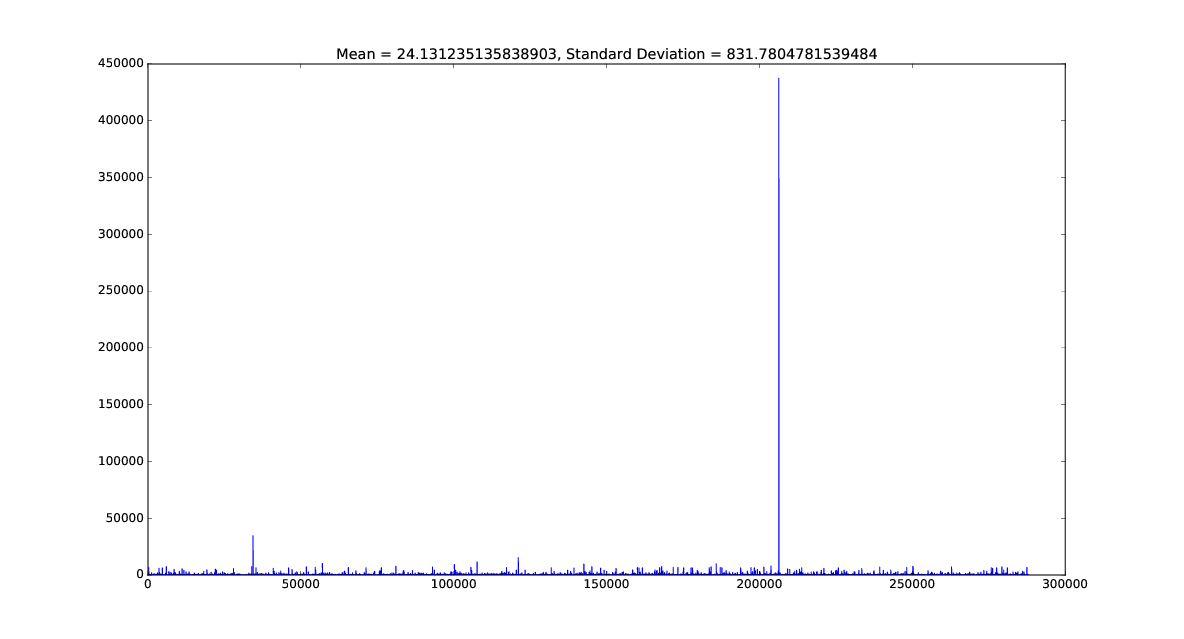
\includegraphics[width=0.75\linewidth]{img/counts_category.png}
\end{figure}
\end{frame}

\begin{frame}
	\frametitle{Verification of network centrality}
\begin{itemize}
\item We run PageRank algorithm on the thresholded, weighted graph.
\item Among the top 20 reported in paper we get 16 same persons in top 20 in our experiments, the rest 4 are within top 30.
\item The exact order among the top-20 is changed, but not drastically.
\end{itemize}
\end{frame}

\begin{frame}
	\frametitle{Communities within the graph}
\begin{itemize}
\item We used Louvain's algorithm for community detection which forms hard clusters, as opposed to SLPA which is a soft clustering algorithm, due to compute constraints.
\item We run the Louvain's algorithm on the thresholded, weighted graph.
\end{itemize}
\resizebox{\textwidth}{!}{
\begin{tabular}{|l|l|l|}
\hline
                   & All communities & Natural Communities  (10 $\leq$ n $\leq$ 50) \\ \hline \hline
F1 Score           & 0.3202          & 0.3985                         \\ \hline
Precision          & 0.8811          & 0.7661                         \\ \hline
Recall             & 0.3547          & 0.7943                         \\ \hline
No. of communities & 7875            & 146                            \\ \hline
\end{tabular}}
\end{frame}

\begin{frame}
	\frametitle{Communities within the graph}
\begin{figure}
	\caption{Variation of the number of detected communities against size}
	\centering
    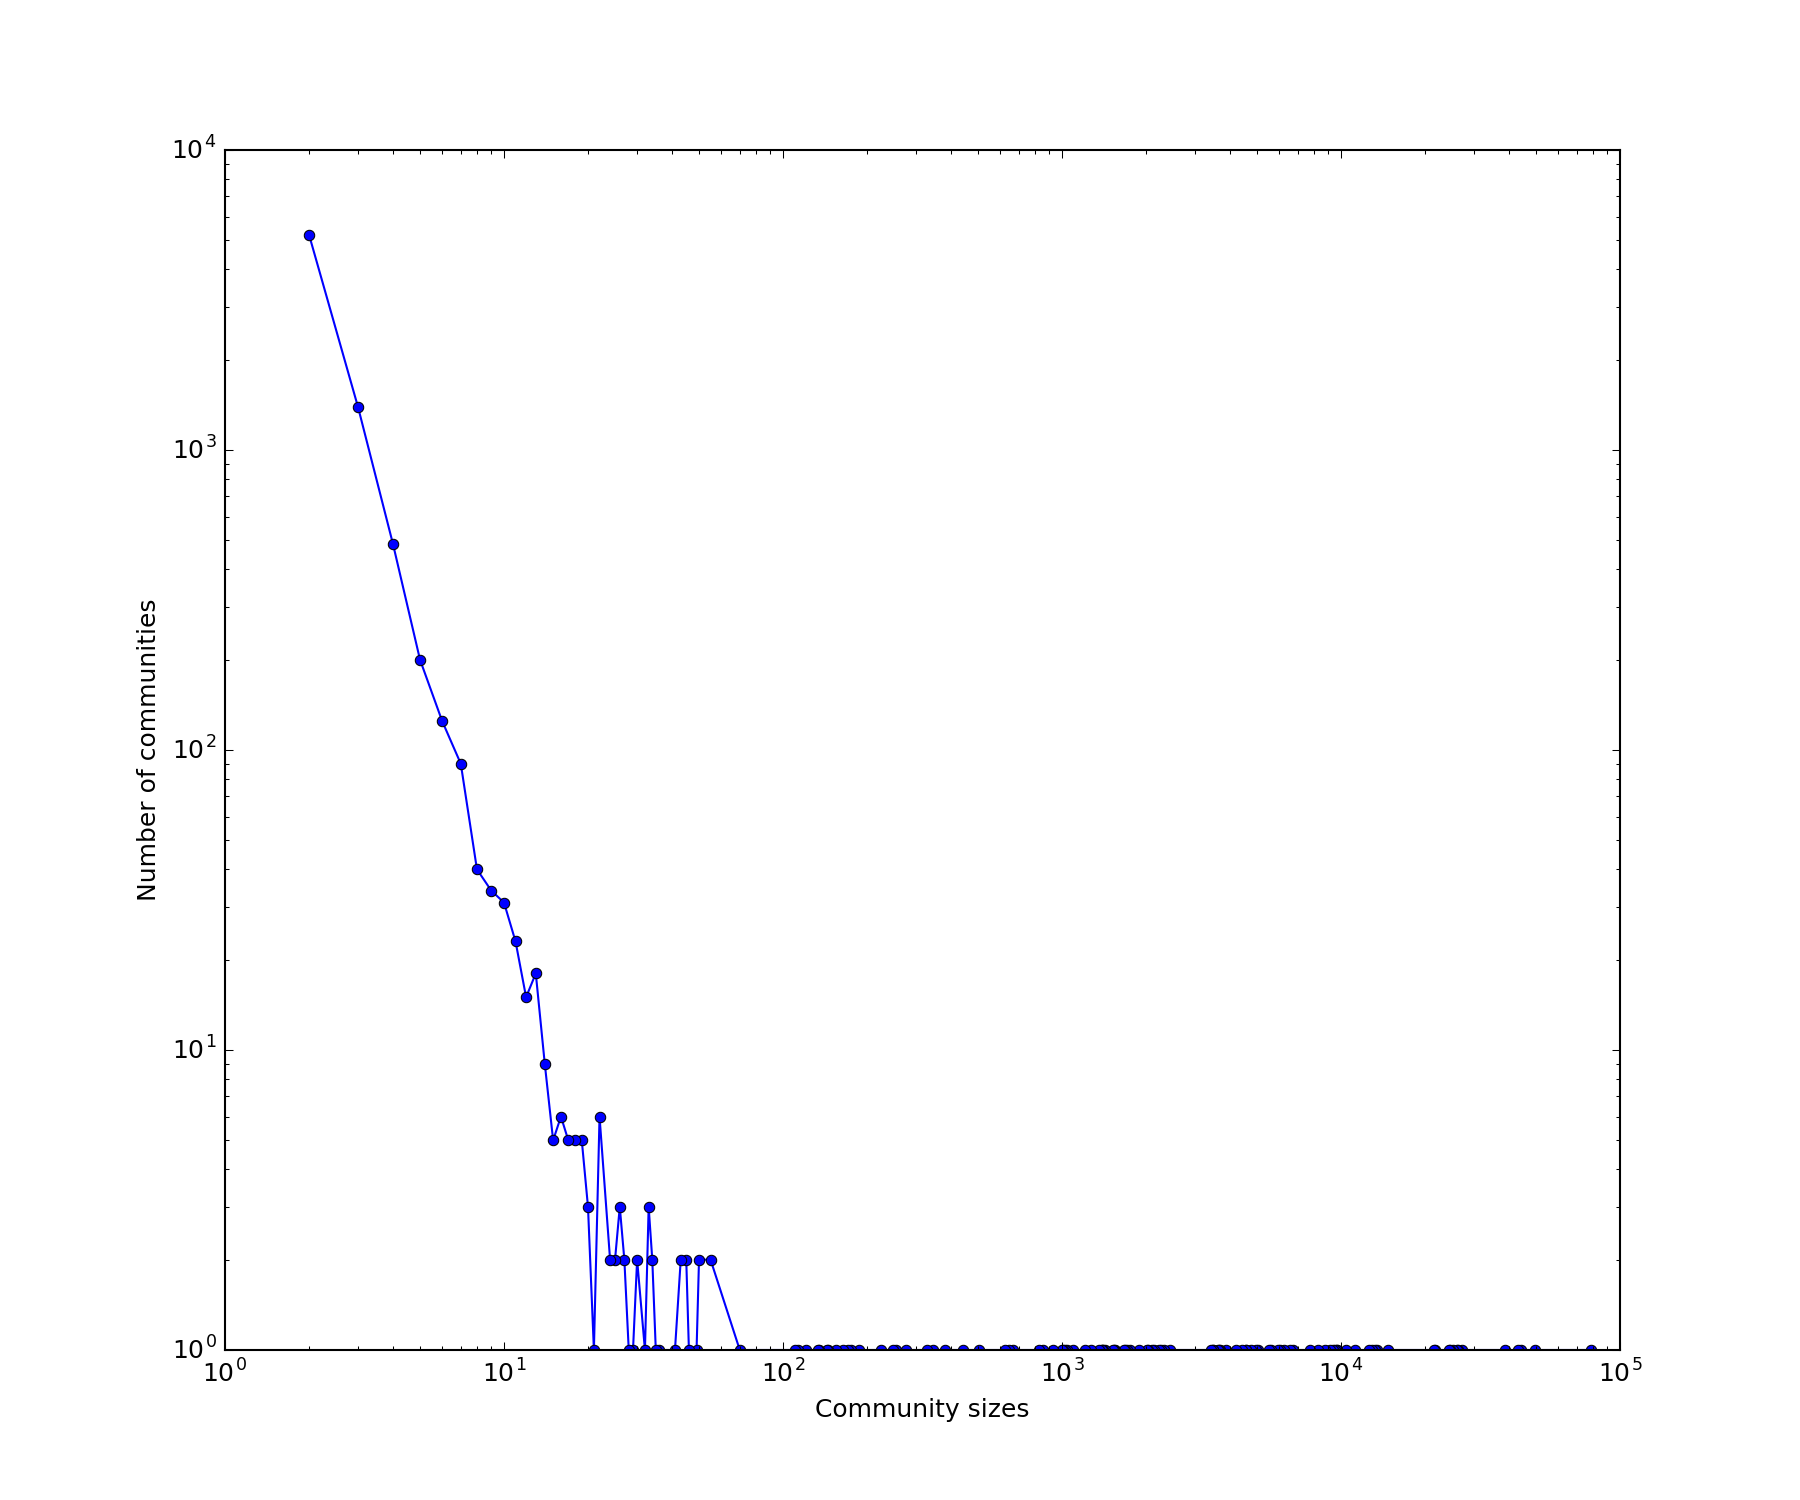
\includegraphics[width=0.75\linewidth]{img/community-counts.png}
\end{figure}
\end{frame}

\begin{frame}[fragile]
	\frametitle{Community-PageRank Pipeline : Motivation}
\vspace{-10mm}
\begin{itemize}
\item Given a page, one would like to assign categories to it.
\item There are two methods:
\begin{itemize}
	\item Extreme-classification: Assign multiple classes to a page from a wide range of classes.
    \item Community-common-categories: Assign a community to a page, get the common categories that the people belong to in that community, and assign it.
\end{itemize}
\item Advantages are that the number of actual classes (here, communities) are relatively low, and is capable of doing multi-category recommendation without as much hassle as extreme classification.
\item Novel too!!
\end{itemize}
\end{frame}

\begin{frame}[fragile]
	\frametitle{Community-PageRank Pipeline}
\vspace{-10mm}
\begin{itemize}
\item Detect communities in the graphs and obtain reasonably sized communities i.e., communities that are not too small.
\item Obtain the top people in these communities and their pages.
\item Use language processing techniques to extract features and subsequently, build a classifier.
\item Given a new page, predict a community.
\end{itemize}
\end{frame}

\begin{frame}[fragile]
	\frametitle{Community-PageRank Pipeline - Community Detection and Filtering}
\vspace{-10mm}
\begin{itemize}
\item We require a scalable algorithm considering the size of the graph.
\item Due to this, we stuck with Louvain's algorithm as used for the verification of results.
\item In our case, we decided from the distribution of the community sizes that minimum size of a reasonably sized community will be 50.
\item Hence we filter out the community whose size is less than 50.
\end{itemize}
\end{frame}

\begin{frame}[fragile]
	\frametitle{Community-PageRank Pipeline - Top People in the Communities}
\vspace{-10mm}
\begin{itemize}
\item We get the top 45 people per community in the filtered out communities.
\item Why 45?
\begin{itemize}
\item Having too low a value will not accommodate for diversity.
\item Having too high a value might corrupt the quality of the features in later phases.
\end{itemize}
\item We use PageRank for this purpose.
\end{itemize}
\end{frame}

\begin{frame}[fragile]
	\frametitle{Community-PageRank Pipeline - Natural Language Processing}
\vspace{-10mm}
\begin{itemize}
\item Before classification, we need to clean up the documents and extract features from it.
\item We do the following preprocessing:
\begin{itemize}
\item Tokenizing the documents.
\item Conversion to lower case.
\item Removal of punctuation.
\item Removal of stop words.
\item Lemmatizing the tokens.
\item Removal of empty tokens.
\end{itemize}
\item To obtain the features from the documents, we now use TF-IDF.
\end{itemize}
\end{frame}

\begin{frame}[fragile]
	\frametitle{Community-PageRank Pipeline - Prediction for a page}
\vspace{-10mm}
\begin{itemize}
\item Now that we know how a page's features are being extracted, we obtain the subset of the entire bunch of features to train a classifier.
\item Considering the sparsity and the non-integral values of the features, we didn't resort to using any tree-based classifier (Decision Trees, Random Forests).
\item We had 5 candidates:
\begin{itemize}
	\item Multinomial Naive Bayes Classifier
    \item Multi-layer Perceptions (Shallow Neural Networks)
    \item Multinomial Logistic Regression
    \item One-vs-All classification with the base classifier as a Binary Logistic Regression model
    \item One-vs-One classification with the base classifier as a Binary Logistic Regression model
\end{itemize}
\end{itemize}
\end{frame}

\begin{frame}[fragile]
	\frametitle{Our Results}
\vspace{-10mm}
\begin{itemize}
\item We assemble our training set as the pages of the top 45 users in each community.
\item The test set is obtained by taking a random 5 among the rest of the users in every community.
\item We do this for three variation of the graphs and community subgraphs
\begin{itemize}
	\item [S1] Community Detection and PageRank with the weighted graph
    \item [S2] Community Detection with the weighted graph and PageRank on the unweighted graph
    \item [S3] Community Detection and PageRank with the unweighted graph
\end{itemize}
\end{itemize}
\begin{center}
\resizebox{\textwidth}{!}{
\begin{tabular}{|c|c|c|c|c}
\cline{1-4}
Scheme & Number of ``valid" communities & Train Set & Test Set & \\
\cline{1-4}
\cline{1-4}
S1 & 106 & 4680 & 530 & \(\Rightarrow\) D1 \\
\cline{1-4}
S2 & 106 & 4511 & 530 & \(\Rightarrow\) D2 \\
\cline{1-4}
S3 & 54 & 2317 & 269 & \(\Rightarrow\) D3 \\
\cline{1-4}
\end{tabular}}
\end{center}
\end{frame}

\begin{frame}[fragile]
	\frametitle{Our Results ... contd..}
Our best and worst accuracies achieved on these datasets are tabulated below:
\begin{center}
\begin{tabular}{|c|c|c|}
\hline
Dataset & Best Test Set Accuracy & Worst Test Set Accuracy \\
\hline
\hline
D1 (with 20000 features) & 66.038\% & 47.925\% \\
\hline
D2 (with 20000 features) & 68.491\% & 45.472\% \\
\hline
D3 (with 10000 features) & 63.941\% & 47.955\% \\
\hline
\end{tabular}
\end{center}
\begin{itemize}
\item The best results were achieved using Multinomial Logistic Regression, One-vs-All Binary Logistic Regression.
\item The worst results were achieved using K-Nearest Neighbours and a 2-hidden layer multi-layer perceptron (optimized using L-BFGS).
\end{itemize}
\end{frame}

\begin{frame}[fragile]
	\frametitle{Our Results ... contd..}
\vspace{-10mm}
\begin{itemize}
\item To test the efficacy of TF-IDF and also to establish certain baselines, we obtain three more set of features from each dataset.
\item These three variants are obtained using top-K term frequencies (TF) and K-randomly picked features from the computed TF-IDF and TF as opposed to best features.
\item The top-K TF-IDF are obtained by checking those K features, which are more correlated with the result.
\item We proceed to train the classifiers with these sets, and the best obtained results are tabulated below.
\end{itemize}
\begin{center}
\resizebox{\textwidth}{!}{
\begin{tabular}{|c|c|c|c|c|c|}
\hline
Dataset & K & Best - TF-IDF & Best - TF & Random - TF-IDF & Random - TF \\
\hline
\hline
D1 & 20000 & 66.038\% & 64.717\% & 10\% & 8.113\% \\
\hline
D2 & 20000 & 68.491\% & 62.830\% & 8.868\% & 7.547\% \\
\hline
D3 & 10000 & 63.941\% & 60.595\% & 10.781\% & 10.409\% \\
\hline
\end{tabular}}

\end{center}
\end{frame}

\begin{frame}[fragile]
	\frametitle{Acknowledgements}
We would like to thank Nagendra Kumar for his valuable guidance and motivation throughout the course of the project.
\end{frame}

\plain{Questions?}
\plain{Thank You.\\\vspace{15mm}Our results are reproducible, so  please check out \texttt{https://github.com/vishwakftw/CS6670-TDM}\\ for the code}
\end{document}